
%(BEGIN_QUESTION)
% Copyright 2007, Tony R. Kuphaldt, released under the Creative Commons Attribution License (v 1.0)
% This means you may do almost anything with this work of mine, so long as you give me proper credit

{\it Derivative} control action is where the output signal of a controller shifts in direct proportion to the rate that {\it error} (the difference between process variable and setpoint) changes.

Given this definition, identify how a derivative-acting controller would respond to the following process variable (PV) and setpoint (SP) values over time:

$$\includegraphics[width=15.5cm]{i02419x01.eps}$$

Assume {\it direct} control action.

\underbar{file i02419}
%(END_QUESTION)





%(BEGIN_ANSWER)

With derivative action, the {\bf rate} at which error moves tells the output how {\bf far} to go:

$$\includegraphics[width=15.5cm]{i02419x02.eps}$$

%(END_ANSWER)





%(BEGIN_NOTES)


%INDEX% Control, derivative: defined

%(END_NOTES)


